\documentclass{instructions}

\usepackage{alltt}
\usepackage{xspace}

\newcommand{\git}{\texttt{git}\xspace}
\newcommand\bs{\char`\\}

\graphicspath{{figs/}}

\title{Practical 4: Controlling the motor}
\date{\today}

\summary{
    For the last week on this DC motor lab, we want to properly control
    the speed of our home-made DC motor with the help of an encoder, and
    H-bridge, and some control logic.
}

\objectives{
At the end of the lab, you should:

\begin{itemize}
    \item have built a proper, closed-loop, motor and controller,
    \item understand what PWM signals and a H-bridge are,
    \item know how to use the Arduino's motor shield.
\end{itemize}
}

\challenges{

    \begin{itemize}
        \item This last lab is really about integration: you'll need a
            working DC motor and a working encoder.
        \item Besides wiring these components together, this lab mainly requires
            you to program the Arduino.
    \end{itemize}
}

\begin{document}

\maketitle


\note{
In your lab journal, \textbf{describe the basic design of each component},
\textbf{how it was constructed} and \textbf{how it was tested}. Add
\textbf{pictures} and link to \textbf{videos} as needed.

Describe as well \textbf{the overall system} and how it performs.

\vspace{1em}

And do not forget: \textbf{write your lab journal as a text file using the Markdown
syntax} and \textbf{push your journal and the pictures on GitHub}.

}

%%%%%%%%%%%%%%%%%%%%%%%%%%%%%%%%%%%%%%%%%%%%%%%%%%%%%%%%%%%%%%%%%%
%%%%%%%%%%%%%%%%%%%%%%%%%%%%%%%%%%%%%%%%%%%%%%%%%%%%%%%%%%%%%%%%%%
%%%%%%%%%%%%%%%%%%%%%%%%%%%%%%%%%%%%%%%%%%%%%%%%%%%%%%%%%%%%%%%%%%

\pagebreak

\intro

\step{Sign-out an Arduino + motor shield kit}

Sign-out and collect from SMB310 an Arduino Uno Kit (Arduino Uno, power supply,
motor shield).

You can keep it for as long as you need to finish all the laboratory sessions.

Return the kit (before the end of term!) when you are done.

\step{Finish your DC motor and encoder}

\important{
    This last 'DC motor' lab is about integrating the motor and the encoder
    together with the Arduino's motor shield to program a closed-loop motor
    controller.

    \textbf{You need a working DC motor and encoder}. Finish first the previous
    labs and ask for help if you are really late.
}


\part{Controlling a small hobby motor}

\step{Install the motor shield}

\begin{figure}[h!]
    \centering
    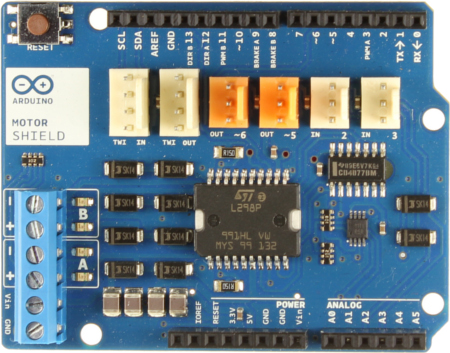
\includegraphics[width=0.6\linewidth]{motorshield}
    \caption{Motor shield. The motor screw terminal connection block is found on
the left}
    \label{motorshield}
\end{figure}

This part of this lab is to get you to program an Arduino Uno in conjunction
with a motor shield (Figure~\ref{motorshield}) to control a DC motor.


\begin{figure}
    \centering
    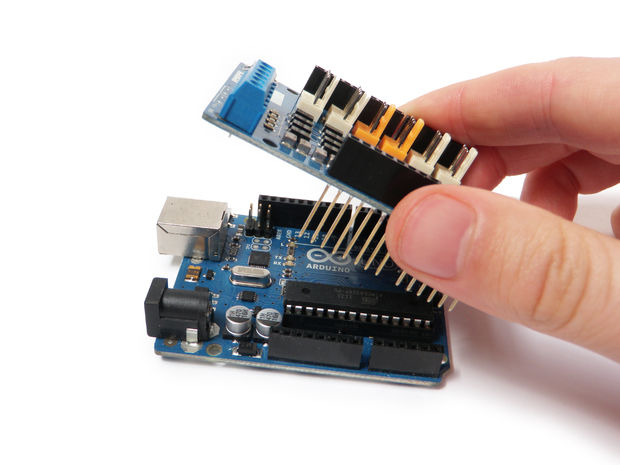
\includegraphics[width=0.45\linewidth]{motorshield-assembly}
    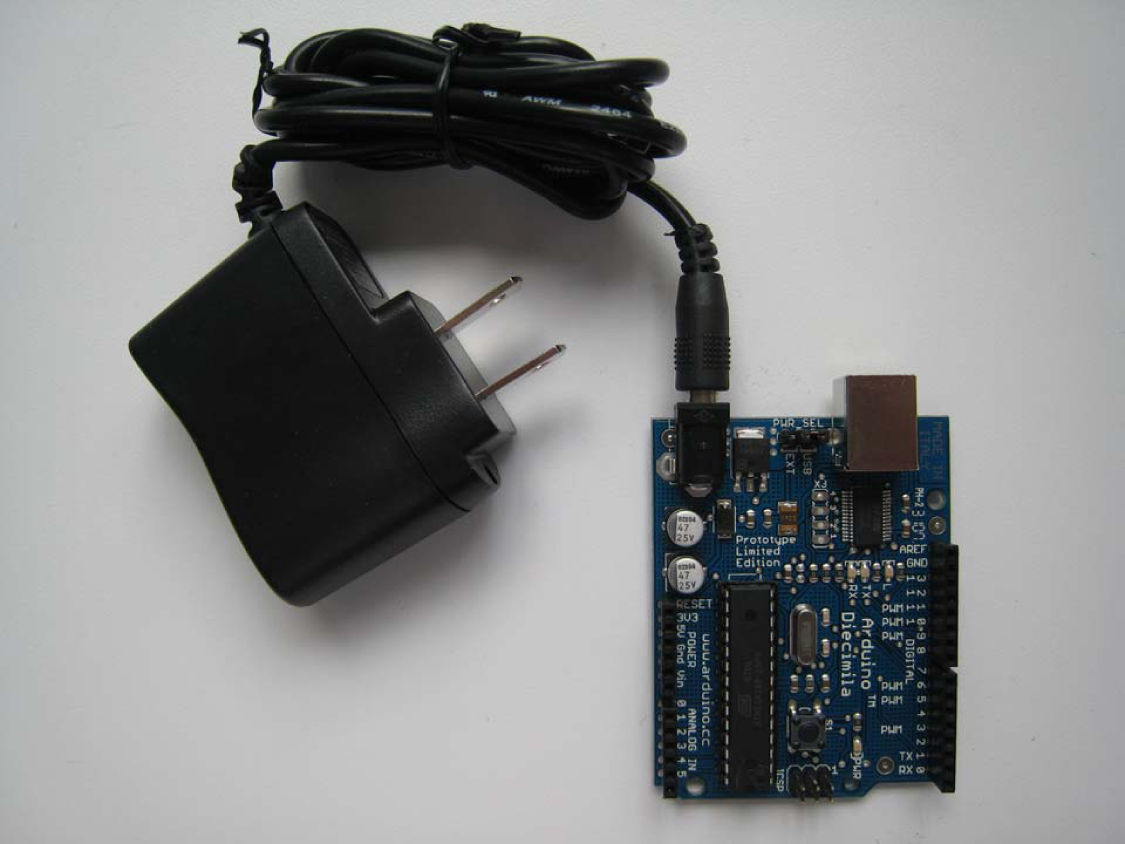
\includegraphics[width=0.45\linewidth]{arduino-powersupply}
    \caption{Assembly of the motor shield on top of the Arduino. On the left,
    the Arduino power supply.}
    \label{assembly}
\end{figure}

First, carefully install the motor shield into the Arduino Uno as shown in
Figure~\ref{assembly}. \textbf{Please ask for help if you aren’t sure what to
do!}

Then, plug in the external power supply. \textbf{Please do not use any other
sources of power yet!} We don’t want to risk damaging to the boards. We need to use
the mains DC power adaptor as the USB power will be insufficient to run the DC
motor.

\step{Control a small hobby DC motor}


\begin{figure}
    \centering
    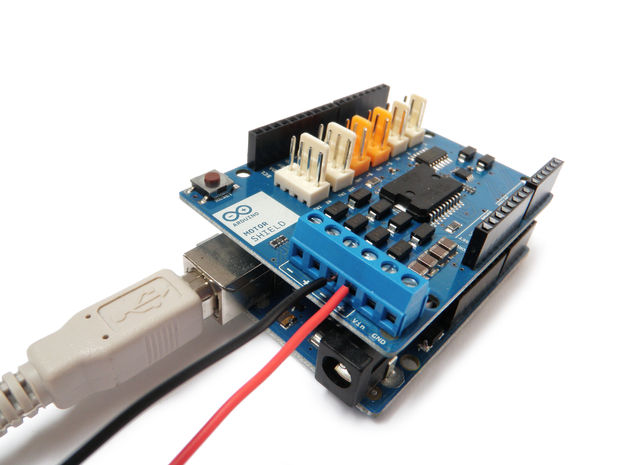
\includegraphics[width=0.5\linewidth]{motor-connection}
    \caption{Motor connected to channel A}
    \label{connection}
\end{figure}

Connect the provided DC motor to the channel A of the motor shield (see
Figure~\ref{connection}). If needed, solder first wires to the motor.

Open the Arduino IDE, plug the provided Arduino, and make sure the IDE is
correctly configured for your card (check the card type -- Arduino UNO -- and
the port -- likely \texttt{/dev/ttyACM0}).


Use the following program to get your hobby motor to turn:

\begin{cppcode}
/*************************************************************
Motor Shield 1-Channel DC Motor
by Randy Sarafan

For more information see:
https://www.instructables.com/id/Arduino-Motor-Shield-Tutorial/
*************************************************************/

void setup() {
  
  //Setup Channel A
  pinMode(12, OUTPUT); //Initiates Motor Channel A pin
  pinMode(9, OUTPUT); //Initiates Brake Channel A pin
  
}

void loop(){
  
  //forward @ full speed
  digitalWrite(12, HIGH); //Establishes forward direction of Channel A
  digitalWrite(9, LOW);   //Disengage the Brake for Channel A
  analogWrite(3, 255);   //Spins the motor on Channel A at full speed
  
  delay(3000);
  
  digitalWrite(9, HIGH); //Eengage the Brake for Channel A

  delay(1000);
  
  //backward @ half speed
  digitalWrite(12, LOW); //Establishes backward direction of Channel A
  digitalWrite(9, LOW);   //Disengage the Brake for Channel A
  analogWrite(3, 123);   //Spins the motor on Channel A at half speed
  
  delay(3000);
  
  digitalWrite(9, HIGH); //Eengage the Brake for Channel A
  
  delay(1000);
  
}
\end{cppcode}

\note{
In your lab journal, describe how one configure and use the Arduino motor
shield: what is the required setup? How to change the rotation direction? How
to change the speed?
}

\part{Controlling your DC motor in closed-loop}


\step{Get your DC motor to rotate}

Now, replace the small provided DC motor by your own motor. You might need to
provide more current: use the lab power supply to power the motor shield, but
\textbf{set the maximum current to 2A} and \textbf{do not exceed 12V}, otherwise
you will damage the motor shield.

\step{Close the loop}

Using your encoder and the Arduino program you wrote last week to read the
speed, write a new program that allow to set the desired speed of the motor in
RPM, and accordingly control the motor.

\note{
Do not forget to document the process!

Insert the code samples (including initial versions which did not work as
expected) in your journal. You can even get syntax highlighting by putting your
the code inside a pre-formatted Markdown block like this one:

\begin{alltt}
```c

// ...

void loop() {

   // ...

}

```

\end{alltt}
}

\end{document}
